\textbf{Pour cette première partie, aucune justification n'est demandée et une seule réponse est possible par question. Pour chaque question, reportez son numéro sur votre copie et indiquez votre réponse.}

Une réponse fausse ou l'absence de réponse n'enlève aucun point.

\needspace{10\baselineskip}
\subsection*{Question 1}

On considère la fonction $f$ définie sur $\R$ par $f(x) = (x-1)^2-8$.

La forme développée de l'expression $f(x)$ est :

\medskip
\begin{tblr}{colspec = {@{}*{4}{X}}}
	\textbf{A.}\quad $x^2-2x-7$ &
	\textbf{B.}\quad $x^2-7$ &
	\textbf{C.}\quad $x^2-9$ &
	\textbf{D.}\quad $x^2-2x-9$ \\
\end{tblr}

\needspace{10\baselineskip}
\subsection*{Question 2}

Le prix de revente d'un véhicule neuf a baissé de 20\,\% la première année puis de 10\,\% la deuxième année. En deux ans, le prix de ce véhicule a :

\medskip
\begin{tblr}{colspec = {@{}*{4}{X}}}
	\textbf{A.}\quad baissé de 30\,\% &
	\textbf{B.}\quad baissé de 72\,\% &
	\textbf{C.}\quad augmenté de 72\,\% &
	\textbf{D.}\quad baissé de 28\,\% \\
\end{tblr}

\needspace{10\baselineskip}
\subsection*{Question 3}

\noindent
\begin{minipage}[c]{0.52\linewidth}
	On donne ci-contre la courbe représentative $\mathcal{C}_f$ d'une fonction $f$ définie sur l'intervalle $[-6 ; 7]$.

	\medskip
	On considère l'équation $f(x) = 0$.

	\medskip
	On peut affirmer que :

	\medskip
	\begin{tblr}{colspec = {@{}X}}
		\textbf{A.}\quad l'équation admet deux solutions positives \\
		\textbf{B.}\quad l'équation admet exactement deux solutions \\
		\textbf{C.}\quad l'équation n'admet pas de solution \\
		\textbf{D.}\quad l'équation admet exactement une solution positive \\
	\end{tblr}
\end{minipage}
\hfill
\begin{minipage}[c]{0.45\linewidth}
	\centering
	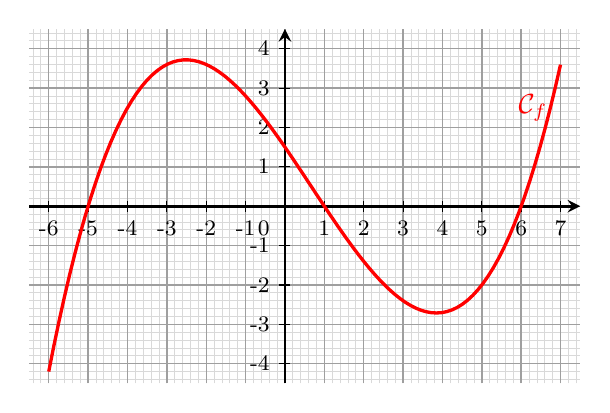
\begin{tikzpicture}[x=0.5cm,y=0.5cm,>=stealth]
		\draw[step=0.2,gray!30,line width=0.3pt] (-6.5,-4.5) grid (7.5,4.5);
		\draw[step=1,gray!75,line width=0.5pt] (-6.5,-4.5) grid (7.5,4.5);
		\draw[->,line width=1pt] (-6.5,0) -- (7.5,0);
		\draw[->,line width=1pt] (0,-4.5) -- (0,4.5);
		\foreach \x in {-6,-5,-4,-3,-2,-1,1,2,3,4,5,6,7} \draw (\x,2pt) -- (\x,-2pt) node[below] {\footnotesize \np{\x}};
		\foreach \y in {-4,-3,-2,-1,1,2,3,4} \draw (2pt,\y) -- (-2pt,\y) node[left] {\footnotesize \np{\y}};
		\draw (-2pt,-2pt) node[below left] {\footnotesize 0};
		\draw[line width=1.2pt,red] plot[domain=-6:7,samples=100] (\x,{0.05*(\x+5)*(\x-1)*(\x-6)});
		\node[red] at (6.3,2.5) {$\mathcal{C}_f$};
	\end{tikzpicture}
\end{minipage}

\needspace{10\baselineskip}
\subsection*{Question 4}

Soit $(d)$ la droite représentée dans le repère orthonormé ci-dessous.

\begin{center}
	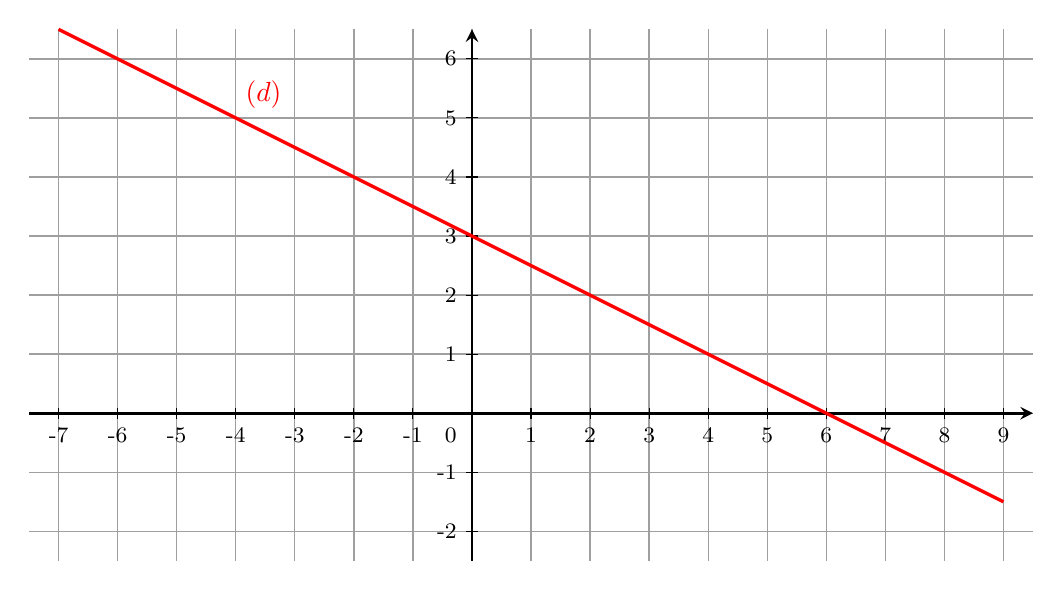
\begin{tikzpicture}[x=0.75cm,y=0.75cm,>=stealth]
		\draw[step=1,gray!75,line width=0.5pt] (-7.5,-2.5) grid (9.5,6.5);
		\draw[->,line width=1pt] (-7.5,0) -- (9.5,0);
		\draw[->,line width=1pt] (0,-2.5) -- (0,6.5);
		\foreach \x in {-7,-6,-5,-4,-3,-2,-1,1,2,3,4,5,6,7,8,9} \draw (\x,2pt) -- (\x,-2pt) node[below] {\footnotesize \np{\x}};
		\foreach \y in {-2,-1,1,2,3,4,5,6} \draw (2pt,\y) -- (-2pt,\y) node[left] {\footnotesize \np{\y}};
		\draw (-2pt,-2pt) node[below left] {\footnotesize 0};
		\draw[line width=1.2pt,red] plot[domain=-7:9] (\x,{-0.5*\x+3});
		\node[above right,red] at (-4,5) {$(d)$};
	\end{tikzpicture}
\end{center}

L'équation réduite de la droite $(d)$ est :

\medskip
\begin{tblr}{colspec = {@{}*{4}{X}}}
	\textbf{A.}\quad $y = 3x+6$ &
	\textbf{B.}\quad $y = -2x+3$ &
	\textbf{C.}\quad $y = \dfrac{1}{2}x+6$ &
	\textbf{D.}\quad $y = -\dfrac{1}{2}x+3$ \\
\end{tblr}

\needspace{10\baselineskip}
\subsection*{Question 5}

Le diagramme en barres ci-dessous donne la répartition des hébergements collectifs de tourisme depuis 2013.

\begin{center}
	\begin{tikzpicture}[y=0.012cm,x=0.9cm]
		\foreach \yy in {0,10,...,500} \draw[thin,lightgray] (11,\yy) -- (-0.3,\yy);
		\foreach \y in {0,50,...,500} \draw[gray] (11,\y) -- (-0.3,\y) node[black,left,font=\tiny] {\y};
		\foreach [count=\i from 0] \annee/\h/\c/\a in {2013/202/311/408,2014/204/318/404,2015/204/316/410,2016/203/280/370,2017/211/336/431,2018/218/341/441,2019/219/348/447,2020/118/222/280,2021/90/202/272,2022/212/349/444,2023/219/360/453}{
			\fill[draw,fill=white] (\i,0) rectangle ++(0.7,\h);
			\fill[draw,black] (\i,\h) rectangle ({\i+0.7},\c);
			\fill[draw,fill=white] (\i,\c) rectangle ({\i+0.7},\a);
			\fill[draw,pattern=bricks,pattern color=darkgray] (\i,\c) rectangle ({\i+0.7},\a);
			\node[font=\tiny] at (\i+0.35,-25) {\annee};
		}
		\node[font=\bfseries\sffamily\tiny,rotate=90,anchor=center] at (-1.3,250) {En millions de nuitées};
		\node[font=\bfseries\small\sffamily,above=2mm] at (5,500) {Répartition des hébergements collectifs de tourisme depuis 2013};
		\draw[fill=white] (0,-90) rectangle ++(1em,1em);
		\node[right,font=\sffamily\tiny,text depth=0pt] at ([xshift=1em,yshift=0.5em]0,-90) {\vphantom{g}Hôtels};
		\fill[draw,black] (2.5,-90) rectangle ++(1em,1em);
		\node[right,font=\sffamily\tiny,text depth=0pt] at ([xshift=1em,yshift=0.5em]2.5,-90) {Campings};
		\fill[draw,pattern=bricks,pattern color=gray] (5.5,-90) rectangle ++(1em,1em);
		\node[right,font=\sffamily\tiny,text depth=0pt] at ([xshift=1em,yshift=0.5em]5.5,-90) {Autres hébergements collectifs de tourisme};
	\end{tikzpicture}
\end{center}

L'année où le nombre de nuitées en camping a été le plus faible est :

\medskip
\begin{tblr}{colspec = {@{}*{4}{X}}}
	\textbf{A.}\quad 2020 &
	\textbf{B.}\quad 2016 &
	\textbf{C.}\quad 2021 &
	\textbf{D.}\quad 2014 \\
\end{tblr}

\needspace{10\baselineskip}
\subsection*{Question 6}

On considère le nombre $N = \np{0,026} \times 10^{-3}$.

$N$ est égal à :

\medskip
\begin{tblr}{colspec = {@{}*{4}{X}}}
	\textbf{A.}\quad $2,6 \times 10^{-1}$ &
	\textbf{B.}\quad $\np{0,0026} \times 10^{-4}$ &
	\textbf{C.}\quad $2,6 \times 10^{-5}$ &
	\textbf{D.}\quad 26 \\
\end{tblr}

\needspace{10\baselineskip}
\subsection*{Question 7}

Dans un repère orthonormé on considère les points $A(5 ; 15)$ et $B(7 ; -5)$. Le coefficient directeur de la droite $(AB)$ est :

\medskip
\begin{tblr}{colspec = {@{}*{4}{X}}}
	\textbf{A.}\quad $-10$ &
	\textbf{B.}\quad $-0,1$ &
	\textbf{C.}\quad $\dfrac{5}{6}$ &
	\textbf{D.}\quad $0,1$ \\
\end{tblr}

\needspace{10\baselineskip}
\subsection*{Question 8}

On considère la fonction $f$ définie sur $\R$ par $f(x) = 4x+3$. Son tableau de signes est :

\medskip
\begin{tblr}{colspec = {@{}*{2}{X}}, rowsep=6pt}
	\textbf{A.}\quad
	\begin{tikzpicture}[baseline=(current bounding box.center)]
		\tkzTabInit[espcl=1.75]{$x$/0.8,$f(x)$/1}{$-\infty$,$\frac{3}{4}$,$+\infty$}
		\tkzTabLine{,-,z,+,}
	\end{tikzpicture}
	&
	\textbf{B.}\quad
	\begin{tikzpicture}[baseline=(current bounding box.center)]
		\tkzTabInit[espcl=1.75]{$x$/0.8,$f(x)$/1}{$-\infty$,$-\frac{3}{4}$,$+\infty$}
		\tkzTabLine{,+,z,-,}
	\end{tikzpicture}
	\\
	\textbf{C.}\quad
	\begin{tikzpicture}[baseline=(current bounding box.center)]
		\tkzTabInit[espcl=1.75]{$x$/0.8,$f(x)$/1}{$-\infty$,$4$,$+\infty$}
		\tkzTabLine{,+,z,-,}
	\end{tikzpicture}
	&
	\textbf{D.}\quad
	\begin{tikzpicture}[baseline=(current bounding box.center)]
		\tkzTabInit[espcl=1.75]{$x$/0.8,$f(x)$/1}{$-\infty$,$-\frac{3}{4}$,$+\infty$}
		\tkzTabLine{,-,z,+,}
	\end{tikzpicture}
	\\
\end{tblr}

\needspace{10\baselineskip}
\subsection*{Question 9}

On souhaite exprimer $F = \dfrac{1}{2+\frac{5}{6}}$ sous la forme d'une fraction irréductible.

\medskip
\begin{tblr}{colspec = {@{}*{4}{X}}}
	\textbf{A.}\quad $F = \dfrac{6}{17}$ &
	\textbf{B.}\quad $F = \dfrac{12}{17}$ &
	\textbf{C.}\quad $F = \dfrac{6}{7}$ &
	\textbf{D.}\quad $F = -\dfrac{17}{6}$ \\
\end{tblr}

\needspace{10\baselineskip}
\subsection*{Question 10}

On considère l'équation suivante : $(3x+1)(x-5) = 0$.

Soit $S$ l'ensemble des solutions de cette équation.

\medskip
\begin{tblr}{colspec = {@{}*{4}{X}}}
	\textbf{A.}\quad $S = \left\{-\dfrac{1}{3}~;~5\right\}$ &
	\textbf{B.}\quad $S = \left\{-5~;~\dfrac{1}{3}\right\}$ &
	\textbf{C.}\quad $S = \{-5~;~-3\}$ &
	\textbf{D.}\quad $S = \left\{\dfrac{1}{3}~;~5\right\}$ \\
\end{tblr}

\needspace{10\baselineskip}
\subsection*{Question 11}

\begin{minipage}[t]{0.52\linewidth}
	On considère les fonctions $f$ et $g$ définies sur l'intervalle $[-5 ; 5]$. On donne ci-contre, dans un repère orthonormé, la représentation graphique $\mathcal{C}_f$ de la fonction $f$ et la représentation graphique $\mathcal{C}_g$ de la fonction $g$.

	L'ensemble des solutions de l'inéquation $f(x) \leqslant g(x)$ est :

	\medskip
	\begin{tblr}{colspec = {@{}X}}
		\textbf{A.}\quad $S = [-5~;~-3] \cup [4~;~5]$ \\
		\textbf{B.}\quad $S = \left]-3~;~2\right[$ \\
		\textbf{C.}\quad $S = [-5~;~-3]$ \\
		\textbf{D.}\quad $S = [-5~;~-3] \cup [2~;~5]$ \\
	\end{tblr}
\end{minipage}
\hfill
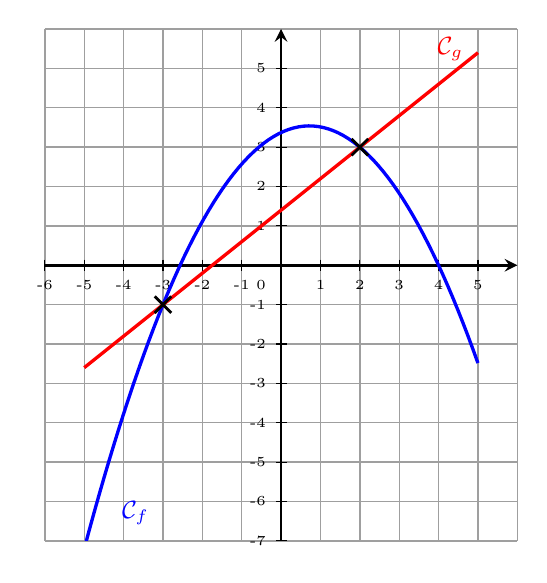
\begin{tikzpicture}[x=0.5cm,y=0.5cm,>=stealth,baseline={(current bounding box.north)}]
	\draw[step=1,gray!75,line width=0.5pt] (-6,-7) grid (6,6);
	\draw[->,line width=1pt] (-6,0) -- (6,0);
	\draw[->,line width=1pt] (0,-7) -- (0,6);
	\foreach \x in {-6,-5,-4,-3,-2,-1,1,2,3,4,5} \draw (\x,2pt) -- (\x,-2pt) node[below] {\tiny \np{\x}};
	\foreach \y in {-7,-6,-5,-4,-3,-2,-1,1,2,3,4,5} \draw (2pt,\y) -- (-2pt,\y) node[left] {\tiny \np{\y}};
	\draw (-2pt,-2pt) node[below left] {\tiny 0};
	\begin{scope}
	\clip (-6,-7) rectangle (6,6);
	\draw[line width=1.2pt,blue] plot[domain=-5:5,samples=80] (\x,{-23/70*(\x-4)*(\x+59/23)});
	\draw[line width=1.2pt,red] plot[domain=-5:5] (\x,{4/5*(\x+3)-1});
	\end{scope}
	\node[blue] at (-3.7,-6.3) {\small $\mathcal{C}_f$};
	\node[red] at (4.3,5.5) {\small $\mathcal{C}_g$};
	\foreach \P in {(-3,-1),(2,3)} \draw[line width=1pt,shift={\P}] (-3pt,-3pt) -- (3pt,3pt) (-3pt,3pt) -- (3pt,-3pt);
\end{tikzpicture}

\needspace{10\baselineskip}
\subsection*{Question 12}

On considère la fonction $f$ définie sur l'intervalle $[-5~;~6]$ et $\mathcal{C}_f$ sa représentation graphique dans le repère ci-dessous.

\begin{center}
	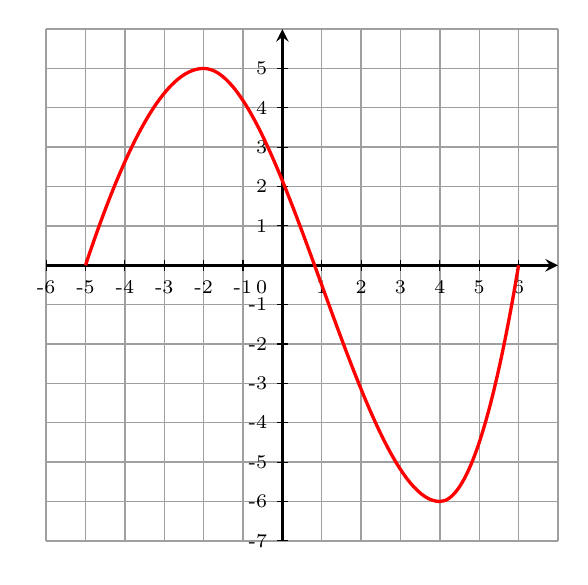
\begin{tikzpicture}[x=0.5cm,y=0.5cm,>=stealth]
		\draw[step=1,gray!75,line width=0.5pt] (-6,-7) grid (7,6);
		\draw[->,line width=1pt] (-6,0) -- (7,0);
		\draw[->,line width=1pt] (0,-7) -- (0,6);
		\foreach \x in {-6,-5,-4,-3,-2,-1,1,2,3,4,5,6} \draw (\x,2pt) -- (\x,-2pt) node[below] {\scriptsize \np{\x}};
		\foreach \y in {-7,-6,-5,-4,-3,-2,-1,1,2,3,4,5} \draw (2pt,\y) -- (-2pt,\y) node[left] {\scriptsize \np{\y}};
		\draw (-2pt,-2pt) node[below left] {\scriptsize 0};
		\draw[line width=1.2pt,red]
		(-5,0) .. controls (-4,3) and (-3,5) ..
		(-2,5) .. controls (0,5) and (2,-6) ..
		(4,-6) .. controls (4.667,-6) and (5.333,-4) .. (6,0);
	\end{tikzpicture}
\end{center}

Le tableau de variations de la fonction $f$ est :

\medskip
\begin{tblr}{colspec = {@{}*{2}{X}}, rowsep=6pt}
	\textbf{A.}\quad
	\begin{tikzpicture}[baseline=(current bounding box.center)]
		\tkzTabInit[lgt=2,espcl=1.375]{$x$/0.6,$f$/1.3}{$-5$,$0$,$4$,$6$}
		\tkzTabVar{-/{$0$},+/{$2{,}5$},-/{$-6$},+/{$0$}}
	\end{tikzpicture}
	&
	\textbf{B.}\quad
	\begin{tikzpicture}[baseline=(current bounding box.center)]
		\tkzTabInit[lgt=2,espcl=1.375]{$x$/0.6,$f$/1.3}{$-5$,$-2$,$4$,$6$}
		\tkzTabVar{-/{$0$},+/{$5$},-/{$-6$},+/{$0$}}
	\end{tikzpicture}
	\\
	\textbf{C.}\quad
	\begin{tikzpicture}[baseline=(current bounding box.center)]
		\tkzTabInit[lgt=2,espcl=1.375]{$x$/0.6,$f$/1.3}{$0$,$5$,$-6$,$0$}
		\tkzTabVar{-/{$-5$},+/{$-2$},-/{$4$},+/{$6$}}
	\end{tikzpicture}
	&
	\textbf{D.}\quad
	\begin{tikzpicture}[baseline=(current bounding box.center)]
		\tkzTabInit[lgt=2,espcl=1.375]{$x$/0.6,$f$/1.3}{$-5$,$1$,$6$}
		\tkzTabVar{-/{$0$},+/{$3$},-/{$0$}}
	\end{tikzpicture}
	\\
\end{tblr}
